

Here, we report detailed results from the models.


\begin{figure}
    \centering
        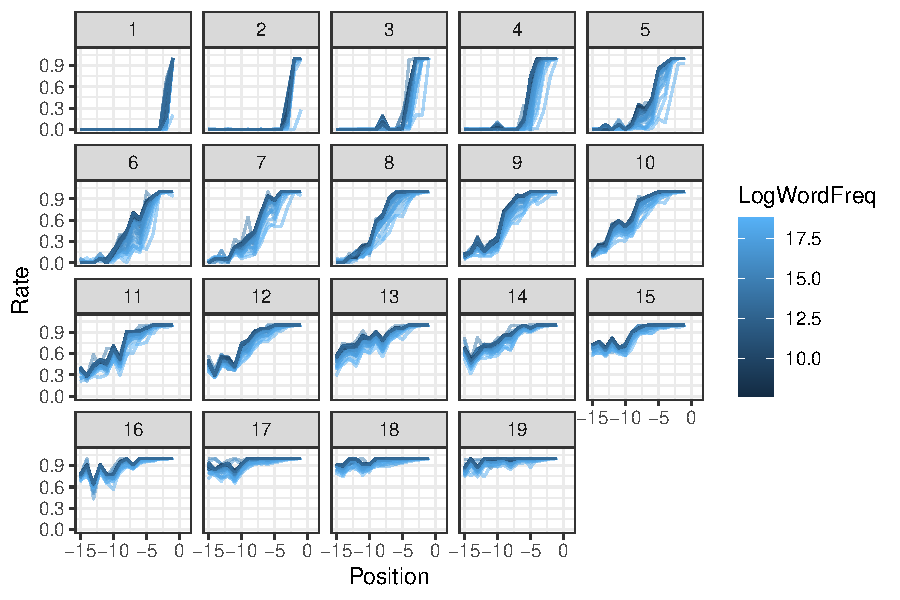
\includegraphics[width=0.7\textwidth]{../resource-rational-surprisal/model/compute_surprisal/figures/retention_rates_lambda1_20_raw_overall.pdf}

    
	\caption{Retention probabilities, as a function of the average number of retained words (``retention rate'', $1 \leq \delta \leq 19$), number of intervening words (x-axis), and log word frequency (color), averaged across all model runs at a given retention rate $\delta$.
	For visibility, we focus on distances $\leq 15$.
	We randomly chose a span of 200 words from the Wikipedia data, held out in the training process. Here, we plot retention probabilities for each word in the span, colored by log word frequency in the Wikipedia corpus. There is a strong recency effect, whereby recent words are more likely to be retained. There furthermore is a frequency effect, whereby lower-frequency words (dark blue) are more likely to be retained.
	Note that the fitted retention probabilities are not fully monotonic as a function of the distance; this can be attributed to the fact that the model has no built-in bias towards progressive decay of representations; this is learnt entirely from the resource-rational objective as applied to the Wikipedia corpus.
	}
    \label{fig:retention-probs}
\end{figure}

\begin{figure}
    \centering
        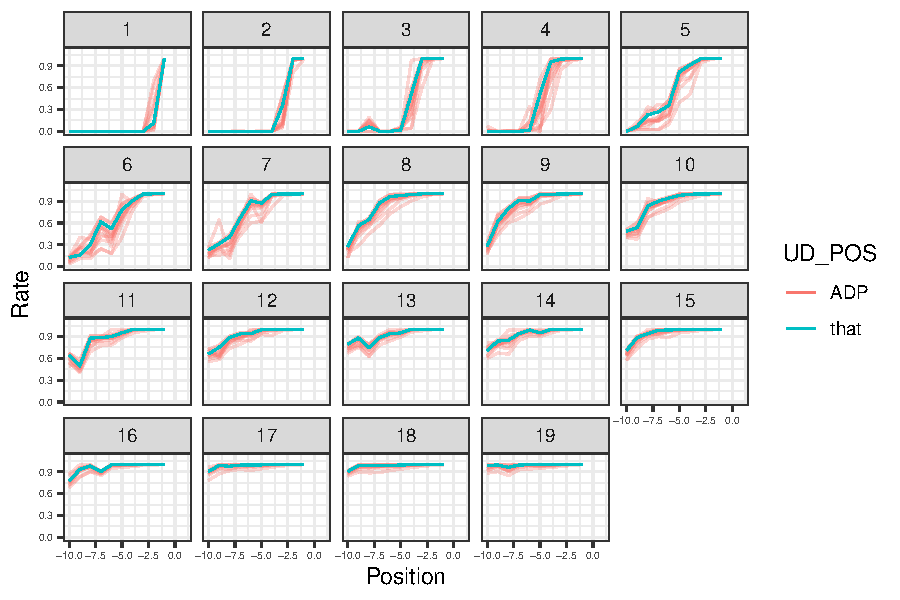
\includegraphics[width=0.7\textwidth]{../resource-rational-surprisal/model/compute_surprisal/figures/retention_rates_lambda1_20_raw_overall_functionWords.pdf}

    
	\caption{Retention probabilities for ``that'' (blue) and for prepositions (red) found in the span of text used for Figure~\ref{fig:retention-probs}.
	For visibility, we focus on distances $\leq 10$.
While both groups of words show very similar trajectories, prepositions have mostly lower retention probabilities than ``that''.
That is, ``that'' is a priori less likely to be forgotten than most prepositions are.
	This means that, when ``that'' has been forgotten, then Bayes's rule (Equation \ref{eq:ref:posterior-bayes}) entails that -- all things being equal -- a higher posterior probability will be assigned to alternative contexts with a preposition (e.g., ``of'', ``by'') in place of ``that''.
	This asymmetry increases the bias towards such structurally different alternatives, unless those have low a-priori probability.
	}
    \label{fig:retention-probs-that}
\end{figure}






\paragraph{Retention Probabilities}
In Figure~\ref{fig:retention-probs}, we plot retention probabilities as a function of word frequency.
There is a recency bias, whereby more recent words have higher retention probabilities.
There is also a word frequency effect, such that low-frequency words are more likely to be retained.

We further specifically plot the retention probabilities for the words most pertinent to the phenomena studied in our experiments: ``that'' and prepositions, in Figure~\ref{fig:retention-probs-that}; see caption for details.

\paragraph{Model Surprisal}
In Figure~\ref{fig:model-surprisal}, we show model surprisal on the critical word in the stimuli in Experiments 1--2 across all model parameters (see caption for details).




\paragraph{Model Fit to Reading Times}

In Figure~\ref{fig:fit-critical}, we show model fit to log reading times on the critical words from trial-by-trial mixed-effects models with model surprisal as fixed effect, and random intercepts for nouns, items, and participants.
Model surprisal was averaged across all model runs for each $\delta$.
These models were fitted with lme4~\citep{Bates2014FittingLM} with maximum likelihood.
\footnote{A possible concern with these analyses is that the number of model runs differs between parameter settings, so that surprisal estimates might have lower variance when there are more model runs.
To rule out this concern, we also conducted an analysis with AICs computed for each model run, and then averaged, and found equivalent results.}




\subsection{Differences between \textsc{Two} and \textsc{Three}}
Figure~\ref{fig:model-surprisal} shows that varying the average number of retained words ($\delta$, ``retention rate'') changes the relative strength of effects in \textsc{Two} and \textsc{Three}.
This happens because of floor or ceiling effects when the true structure is essentially always or never reconstructed:
For higher retention rates ($\delta \gtrapprox 10$), effects of compatibility and embedding bias are stronger in \textsc{Three} than in \textsc{Two}; this happens because the \textsc{Two} condition is unaffected by memory loss at high retention rates. 
In contrast, for low retention rates, effects of compatibility and embedding bias are stronger in \textsc{Two}, because the syntactic structure is rarely reconstructed correctly in the \textsc{Three} condition. 
Human reading times show stronger effects in \textsc{Three} than in \textsc{Two}, as shown by interactions \textsc{Depth}:\textsc{EmbeddingBias} and \textsc{Depth}:\textsc{Compatibility} in a meta-analysis across reading times (Figure~\ref{fig:meta} in Section~\ref{sec:meta}), suggesting that effects of memory limitations are relatively mild in the \textsc{Two} condition.
This agrees with model behavior at higher average retention rates (e.g., $\delta \approx 10, \dots, 13$ in Figure~\ref{fig:model-surprisal}).
However, the fact that effects of embedding bias and compatibility can be shown individually in human reading times even within the  \textsc{Two} condition  (``FactReportDifferenceTwo'' and ``CompatibilityEffect\_Two'' in Figure~\ref{fig:meta}) shows that this is not a categorical difference: Similar to the behavior of the model, humans are impacted by memory limitations even in the simple \textsc{Two} condition, albeit to a lesser degree than in the more difficult \textsc{Three} condition.
A prediction of the model is thus that, in situations where comprehenders are more forgetful or less attentive, effects should increase within \textsc{Two} and decrease within \textsc{Three}.\footnote{Cf \citet{Nicenboim2016WhenHR} for conceptually related experimental findings, where locality effects increased for high-capacity readers in an experiment in Spanish.}





\begin{figure}
    \centering

	\textbf{Experiment 1}
    
		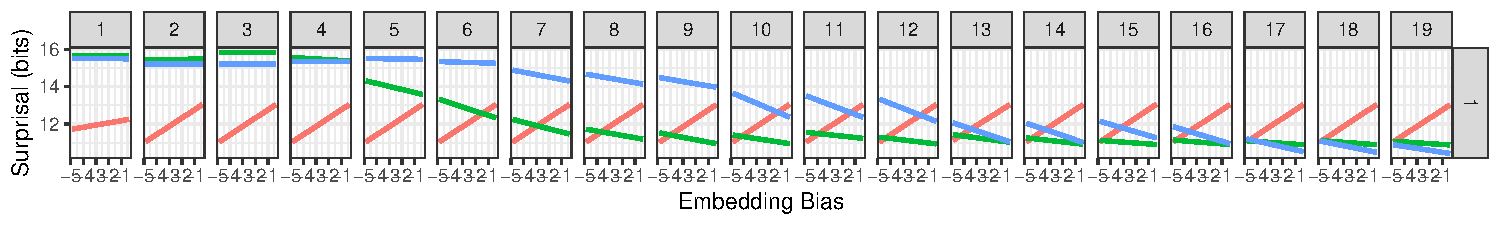
\includegraphics[width=0.8\textwidth]{../resource-rational-surprisal/model/compute_surprisal/analyze_output/figures/model-critical-experiment1-full-NoLimit_Lambda1_Integer_Bits.pdf} %&

	\textbf{Experiment 2}


    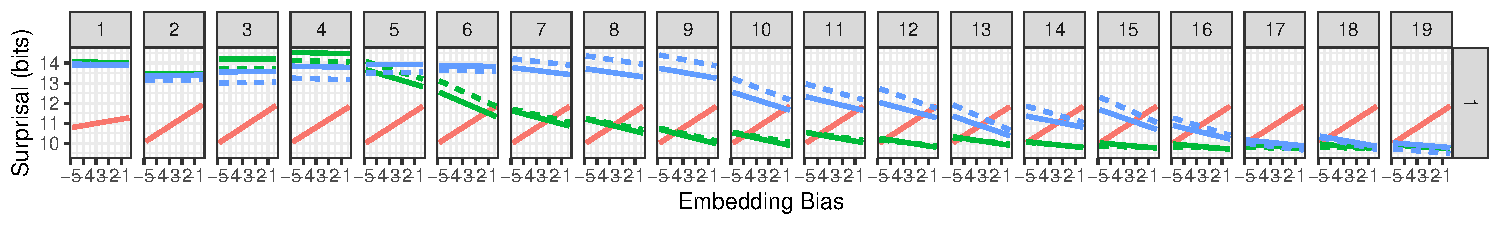
\includegraphics[width=0.8\textwidth]{../resource-rational-surprisal/model/compute_surprisal/analyze_output/figures/model-critical-experiment2-full-NoLimit_Lambda1_Integer_Bits.pdf}


        \begin{tabular}{llllllll}
\textbf{\textcolor{one}{----}} \textsc{One}&
\textbf{\textcolor{two}{----}} \textsc{Two}&
\textbf{\textcolor{three}{----}} \textsc{Three}
\end{tabular}
    
    \begin{tabular}{llllllll}
\textbf{{----}} \textsc{Incompatible}&
\textbf{{- - -}} \textsc{Compatible}
\end{tabular}
    
    
    
   
	\caption{Model surprisal on the final verb across values of the average number of retained words $\deletionRate$ (``retention rate''). We show linear fits across all item-noun-pairs, averaged across all model runs at a given $\delta$.
	}
    \label{fig:model-surprisal}
\end{figure}


\begin{figure}
    \centering


    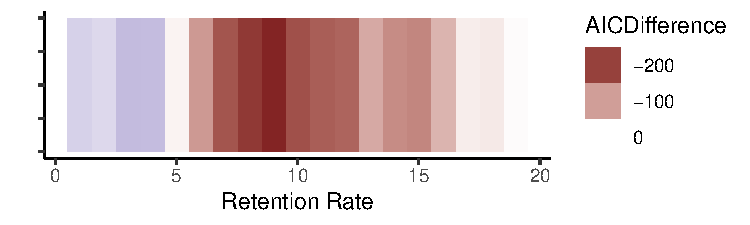
\includegraphics[width=0.6\textwidth]{../resource-rational-surprisal/experiments/maze/meta/figures/analyze_Model_IncludingNoTP_E12_Viz_R_AICRaw_Lambda1_Integer.pdf}


	\caption{Model fit to critical log RTs measured by AIC as a function of the retention rate $\deletionRate$, for the data from Experiments 1 and 2. Compare Figure~\ref{fig:model-surprisal}.
	Model fit is computed using frequentist mixed-effects models with model surprisal as fixed effects predictor, and random intercepts for nouns, items, and participants (see text for details).
	Model fit is compared to the AIC achieved by plain GPT-2 surprisal; negative values indicate a better model fit than GPT-2.
	Fit substantially improves over GPT-2 throughout the range where the three predictions described in the main paper are borne out  (compare Figure~\ref{fig:model-surprisal}).
		}
    \label{fig:fit-critical}
\end{figure}





\begin{figure}
    \centering


    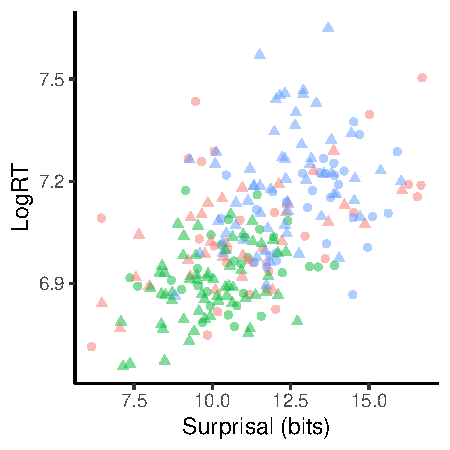
\includegraphics[width=0.6\textwidth]{../resource-rational-surprisal/experiments/maze/meta/figures/analyze_Model_PlotForExpt12_Joint_ModelHuman_OnlyExpt12_R_Bits.pdf}

        \begin{tabular}{llllllll}
\textbf{\textcolor{one}{----}} \textsc{One}&
\textbf{\textcolor{two}{----}} \textsc{Two}&
\textbf{\textcolor{three}{----}} \textsc{Three}
\end{tabular}
 
	\caption{Scaling between surprisal and reading times, at $\delta=10$, for Experiment 1 (circles) and Experiment 2 (triangles). Colors indicate conditions as in the main paper. For each experiment, we plot the mean surprisal and reading time across all trials with a given combination of noun and condition (One/Two/Three crossed with compatibility).
	Scaling of reading times with surprisal is similar in both experiments:
	We conducted Bayesian mixed-effects models predicting log-transformed reading times from model surprisal with a main effect and interaction including the contrast between the two experiments, with full random intercepts and slopes for nouns, items, and participants.
	We found a consistent main effect of surprisal ($\beta=0.066$, 95\% CrI $[0.06, 0.07]$), but no evidence for either a main effect of experiment ($\beta=0.02$, 95\% CrI $[-0.05, 0.1]$) nor for an interaction between surprisal and experiment ($\beta=0.01$, 95\% CrI $[-0.01,0.03]$).
We note that Figure 3 in the main paper might seem to exhibit a difference in the scaling of model surprisal and reading times in the two experiments; this analysis shows that this difference is not statistically meaningful.
	%        sink("output/analyze_Model_IncludingNoTP_E12_Interact.R.txt")   
		}
    \label{fig:fit-critical-scaling-dots}
\end{figure}



\subsection{Uniform Loss Model}

In Figure~\ref{fig:uniform-loss}, we show model surprisal under the assumption of uniform loss, as in the simulations of \citet{Futrell2020LossyContextSA}.
That is, given an average number of retained words, $\delta \in [0,20]$, each word was retained with a uniform probability of $\frac{\delta}{20}$.
The effect of embedding bias is predicted across various values of $\delta$, confirming substantial robustness of this novel prediction.
However, the effects of Compatibility and the \textsc{Two}-\textsc{Three} contrast are predicted inconsistently, sometimes even in the opposite direction from the resource-rational model.
This shows that retention probabilities optimized for the resource-rational objective function match human reading times considerably better than uniform retention probabilities would.


\begin{figure}
    \centering
    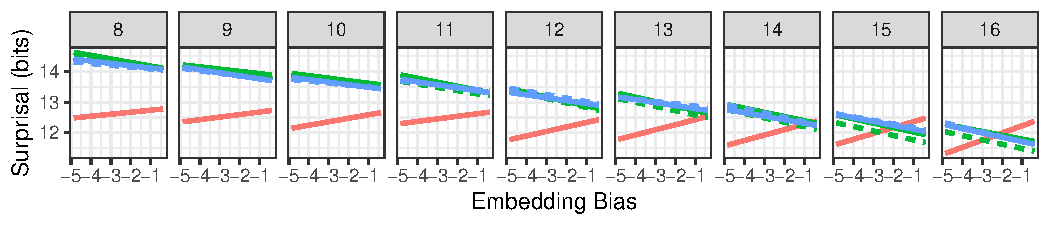
\includegraphics[width=0.8\textwidth]{figures/predictions-surprisal-uniform_Bits.pdf}

        \begin{tabular}{llllllll}
\textbf{\textcolor{one}{----}} \textsc{One}&
\textbf{\textcolor{two}{----}} \textsc{Two}&
\textbf{\textcolor{three}{----}} \textsc{Three}
\end{tabular}
    
    \begin{tabular}{llllllll}
\textbf{{----}} \textsc{Incompatible}&
\textbf{{- - -}} \textsc{Compatible}
\end{tabular}
    
    
 
	\caption{Model surprisal under uniform loss, for different values of $\delta$. The effect of embedding bias is predicted across various values of $\delta$. However, the effects of semantic compatibility and the \textsc{Two}-\textsc{Three} contrast are predicted inconsistently, either with no significant effect or sometimes in the opposite direction compared to the resource-rational model and the human data.}
    \label{fig:uniform-loss}
\end{figure}


We also considered a window-based model where memory representations consist of the past $K = \delta N$ words.
Such a model can account for the effect of depth, but it cannot account for the effect of embedding bias: If the identity of the noun is to impact difficulty, then $K$ must be large enough to include the noun, but then will also include \textit{that}. Therefore, the effect of embedding bias in the presence of a \textit{that}-clause would not arise in such a model.


